\documentclass[border=2pt]{standalone}
\usepackage{tikz}
\usetikzlibrary{arrows.meta,shapes.geometric,topaths}

\begin{document}
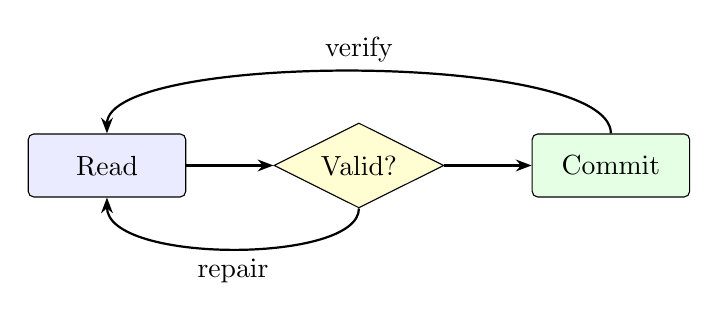
\begin{tikzpicture}[
  stage/.style={draw,rounded corners=2pt,minimum width=20mm,minimum height=8mm,align=center},
  gate/.style={draw,diamond,aspect=2,minimum width=18mm,minimum height=10mm,align=center},
  flow/.style={-{Stealth[length=2mm]},thick}
]
  \node[stage,fill=blue!8] (read) at (0,0) {Read};
  \node[gate,fill=yellow!18] (check) at (3.2,0) {Valid?};
  \node[stage,fill=green!10] (write) at (6.4,0) {Commit};

  \path[flow]
    (read) edge (check)
    (check) edge (write)
    (write) edge[controls={+(0,1.45) and +(0,1.45)}] node[above] {verify} (read)
    (check) edge[out control={+(0,-1.25)},in control={+(0,-1.25)}] node[below] {repair} (read);
\end{tikzpicture}
\end{document}
